\section{Introduction}

%solar wind beginnings
From observations of cometary tail fluctuations \citet{Biermann1951} inferred the presence of a continuous flow of particles from the Sun. With his theoretical solar wind model \citet{Parker1958} formulated the existence of the solar wind even before the first satellites measured it in situ in 1962 \citep{Neugebauer1966} \hl{+ ref. to Russian measurements}.
%in situ spacecraft
The idea of a space mission flying through the solar corona dates back to the founding year of NASA in 1958 \citep{McComas2008}. Since then several space missions have measured the solar wind in situ at a wide range of heliocentric distances, in the case of Voyager~1 as far away as \SI{138}{\au} in July 2017\footnote{\url{https://voyager.jpl.nasa.gov/}}, having even left the heliospause into interstellar space at a distance of \SI{121}{\au} \citep{Gurnett2013}.
Until today various spacecraft have provided a wealth of solar wind measurements near Earth’s orbit, with Wind \hl{(ref.)}, ACE \hl{(ref.)} and DSCOVR \hl{(ref.)} still orbiting around the L1 point \SI{1.5}{million \km} ahead of Earth in the sunward direction. Additional measurements at other distances were provided by planetary missions to Venus and Mercury, such as PVO \hl{(ref.)} or MESSENGER \hl{(ref.)}. Ulysses was the first probe that orbited the Sun out of the ecliptic plane and thus could measure solar wind at polar latitudes \citep{McComas1998}. The nearest in situ solar wind measurements to date were obtained by the Helios mission. The in 1974 launched Helios~1 spacecraft reached distances of \SI{0.31}{\au}, Helios~2 launched two years later and approached the Sun up to \SI{0.29}{\au} \citep{Rosenbauer1977}.

%Solar Probe Plus mission
The NASA Parker~Solar~Probe\footnote{\url{http://parkersolarprobe.jhuapl.edu/}} (PSP), formerly Solar~Probe~Plus, with a planned launch date in mid 2018, will reach after six years in 2024 its closest perihelia at a distance of 9.86~solar radii (\Rsun), that is, \SI{0.0459}{\au} \citep{Fox2015}. This distance will be achieved through seven Venus gravity assists with orbital periods of 88--168~days. In its prime mission time 2018--2025 PSP provides 24~orbits with perihelia inside \SI{0.25}{\au} \citep{Fox2015}. Even its first perihelion, 93~days after launch in 2018, will take PSP to an unprecedented distance of \SI{0.16}{\au} (\SI{35.7}{\Rs}). {\color{Red2} In comparison, the ESA Solar Orbiter mission with a planned launch in 2019 will have a closest perihelion of \SI{0.289}{\au} \hl{(ref.)}.}

%PSP objectives and instruments
The key PSP science objectives are to “trace the flow of energy that heats and accelerates the solar corona and solar wind, determine the structure and dynamics of the plasma and magnetic fields at the sources of the solar wind, and explore mechanisms that accelerate and transport energetic particles” as stated in \citet{Fox2015}. To achieve these goals, PSP has four scientific instruments on board: FIELDS for the measurements of magnetic fields and AC/DC electric fields \citep{Bale2016}, SWEAP for the measurements of flux of electrons, protons and alphas \citep{Kasper2016}, IS\sun{}IS for the measurement of solar energetic particles \citep{McComas2016} and WISPR for the measurement of coronal and inner heliospheric structures \citep{Vourlidas2016}.

%CGAUSS and WISPR
The study presented in this paper is undertaken in the Coronagraphic German And US Solar Probe Survey (CGAUSS) project, which is the German contribution to the PSP mission as part of the Wide field Imager for Solar PRobe (WISPR). WISPR will contribute to the PSP science goals by deriving the 3D structure of the solar corona through which the in situ measurements are made to determine the sources of the solar wind. It will provide density power spectra over a wide range of structures (e.g., streamers, pseudostreamers and equatorial coronal holes) for determining the roles of turbulence, waves and pressure-balanced structures in the solar wind. It will also measure the physical properties, such as speed and density jumps of SEP-producing shocks and their CME drivers as they evolve in the corona and inner heliosphere \citep{Vourlidas2016}.

In order to help optimize the WISPR and PSP preplanning of the science operations knowledge of the expected solar wind environment is needed. For this purpose the solar wind environment is extrapolated down to the closest perihelion of \SI{9.86}{R_s} distance to the Sun using in situ solar wind data from the Helios probes and near \SI{1}{\au} data from various satellites compiled in the NASA/GSFC OMNI solar wind database.\\

%definition of sw environment
%section{Solar wind}

Generally, two types of solar wind are observed in the heliosphere, slow and fast streams \citep{Neugebauer1966}\hl{, Schwenn (19xx)}. Slow solar wind has typical speeds \SI{<400}{\km\per\s} and fast solar wind has speeds \SI{>600}{\km\per\s} \citep[p.~144]{Schwenn1990}. Their different compositions and characteristics indicate different sources and generation processes \citep{McGregor2011a}. Fast streams are found to originate from coronal holes as confirmed by Ulysses out-of-ecliptic measurements \citep{McComas1998}. The source of slow wind and its eventually different types (\hl{Schwenn19xx}), is still a subject of controversial discussions because several scenarios are possible to explain its origin from closed magnetic structures in the solar corona, {\color{red} such as ...intermittent reconnection at the top of streamers and pseudostreamers, coronal hole boundaries, ... (\hl{ref.}).} The occurrence frequency of these slow and fast streams varies strongly with solar activity and their interactions lead to phenomena such as stream interaction regions and for quasi-stationary coronal source regions to co-rotating interaction regions \citep{Balogh1999}.

Embedded in the slow and fast solar wind streams are transient flows of coronal mass ejections (CMEs), the faster ones driving shock waves ahead \hl{(ref.)}. Their rate follows the activity cycle and varies in near \SI{1}{\au} measurements between only one CME every couple of days during solar cycle minima up to multiple CMEs observed over several days at times of solar maxima, that is, the CME-associated flow share of the solar wind raises from about \SI{5}{\percent} up to about \SI{50}{\percent} \citep{Richardson2012}.

It is not known which specific solar wind type or structure PSP will encounter at a given time during its mission, therefore we extrapolate the probability distributions of the major solar wind parameters from existing solar wind measurements and take solar cycle dependencies into account.

%solar wind parameters
As a baseline we describe the solar wind environment through the key quantities of a magnetized plasma: \textit{density}, \textit{temperature} and \textit{magnetic field strength}. Furthermore, the bulk flow \textit{velocity} is the defining parameter of the two types of solar wind. Solar wind quantities, like flux densities, mass flux and plasma beta, can directly be derived from these four parameters.

Our approach is to obtain analytical representations of the shapes of the solar wind parameter’s frequency distributions in Sect.~\ref{sec:frequency_distribution}, of their solar activity dependence in Sect.~\ref{sec:solar_activity_variations} and of their solar distance scaling in Sect.~\ref{sec:solar_distance_dependency}. The solar wind parameters’ frequency distributions and solar activity dependence is derived from near-Earth solar wind and sunspot number (SSN) time series with a duration of almost five solar cycles. Their distance dependency is derived from Helios solar wind measurements covering more than two third of the distance to the Sun and more than half a solar cycle. From combination of the obtained frequency distributions, SSN dependence functions and solar distance dependence functions a general solar wind model is build in Sect.~\ref{sec:general_solar_wind_model}, representing the solar activity and distance behavior. Finally, this empirical model is fed with a SSN prediction and extrapolated to PSP's planned orbital positions in Sect.~\ref{sec:model_extrapolation_to_psp_orbital_time_and_position}.


%lognormal fitting
\section{Frequency distributions of the solar wind parameters}
\label{sec:frequency_distribution}

The solar wind parameters are highly variable, due to short-term variations from structures like slow and fast wind streams, interaction regions and CMEs, whose rate and properties depend on the phase of the solar activity cycle. Hence, for deriving characteristic frequency distributions for the solar wind parameters, measurements over long-term time spans are needed. The abundance of the near-Earth hourly OMNI data set is ideally suited for this purpose, because it spans to date almost five solar cycles.

%about OMNI data
The OMNI~2 data set \citep{King2005} combines solar wind plasma and magnetic field data collected by various satellites since 1963. This intercalibrated multi-spacecraft data is time-shifted to the nose of the Earth’s bow shock. The data is obtained from the OMNIWeb interface\footnote{\url{http://omniweb.gsfc.nasa.gov/}} at NASA's Space Physics Data Facility (SPDF), Goddard Space Flight Center (GSFC).
%OMNIWeb Data Documentation: http://omniweb.gsfc.nasa.gov/html/ow_data.html
% Acknowledgement to the SPDF OMNIWeb database as the source of data used in publications is requested: "The OMNI data were obtained from the GSFC/SPDF OMNIWeb interface at http://omniweb.gsfc.nasa.gov". Further, for recent years when few sources (IMP 8, Wind, ACE, Geotail) contributed to OMNI, it would be appropriate to also cite the PI's who provided the data to OMNI. Copies of preprints or reprints of OMNI-based publications sent to Natalia Papitashvili (address below) would be appreciated for tracking purposes.
% The best citable reference to OMNI data is J.H. King and N.E. Papitashvili, Solar wind spatial scales in and comparisons of hourly Wind and ACE plasma and magnetic field data, J. Geophys. Res., Vol. 110, No. A2, A02209, 10.1029/2004JA010804.
%
%data time range
In this study the whole hourly data until 31 December 2016 is used, starting from 27 November 1963 (for the temperature from 26 July 1965). The data coverage of the parameters is in the range \SIrange{67}{74}{\percent},  corresponding to a total duration of 36--40~years.
%OMNI 1963-01-01 data
%B 1963-11-27 14:30
%V 1963-11-27 12:30
%N 1963-11-27 12:30
%T 1965-07-26 00:30
%1963-01-01~00:00--2016-12-31~23:30 all
%19724 d; 54 y\\
% B: 73.91 \%		39.91 y\\
% V: 73.07 \%		39.46 y\\
% N: 70.29 \%		37.96 y\\
% T: 66.73 \%		36.03 y\\
%
%hourly data
It should be noted that a test-comparison of hourly averaged with higher time resolution data for the available shorter time span 1981--2016, did not show significant differences in our results.

%data binning
The frequency distributions of the solar wind magnetic field strength, proton velocity, density and temperature are shown in Fig.~\ref{fig:histogram_fits_4_a_zoom_paper_pdfplot}. According to the OMNI data precision and maximal parameter ranges we specify the bin sizes to \SI{0.5}{\nT} for the magnetic field strength, \SI{10}{\km\per\s} for the velocity, \SI{1}{\per\cm\cubed} for the density and \SI{10000}{\K} for the temperature.

The solar wind magnetic field strength is in the range \SIrange{0.4}{62}{nT}, the velocity in the range \SIrange{156}{1189}{\km\per\s}, the density in the range \SIrange{0}{117}{\per\cm\cubed}, and the temperature in the range \SIrange{3450}{6.63e6}{\K}, the mean values are at \SI{6.28}{\nT}, \SI{436}{\km\per\s}, \SI{6.8}{\per\cm\cubed} and \SI{1.05e5}{\K}. These ranges and mean values are as statistically expected from previous analyses of near \SI{1}{\au} solar wind data (e.g., Table~3.3 in \citet[p.~39]{Bothmer2007}).

Much higher or lower peak values at \SI{1}{\au} have been observed in extraordinary events, such as the 23~July 2012 ICME with a speed of over \SI{2000}{\km\per\s} and a peak field strength of about \SI{100}{\nT} that was observed by STEREO~A \citep{Russell2013} or the solar wind disappearance event observed in May 1999 with density values even down to \SI{0.2}{\per\cm\cubed} \citep{Lazarus2000}.\\

%subsection{Lognormal fitting}
%choice of distribution function
The frequency distributions of the solar wind parameters magnetic field strength, proton density and temperature can
well be approximated by lognormal distributions, whereas the proton velocity’s frequency has a differing shape, as shown in \citet{Veselovsky2010}. We investigate how well all four solar wind parameters’ frequency distributions can be represented by lognormal functions, which we use in the process of a least squares regression fitting. The lognormal function 
\begin{align}
	W(x) &= \frac{1}{\sigma \sqrt{2 \pi} x} \, \exp\left(- \frac{\left(\ln x - \mu\right)^2}{2 \sigma^2}\right)	\label{eq:lognormal_function}
\end{align}
depends on the location $\mu$ and the shape parameter $\sigma$. Changes in $\mu$ affect both the horizontal and vertical scaling of the function whereas $\sigma$ influences its shape. The distribution's median $x_\text{med}$ and mean $x_\text{avg}$ (average) positions are straightforward to interprete and are directly calculated from $\mu$ and $\sigma$:
\begin{align}
	x_\text{med} &= \exp\left(\mu\right)	&	&\Longleftrightarrow	&	\mu &= \ln\left(x_\text{med}\right)\,,	\label{eq:lognormal_median}\\
	x_\text{avg} &= \exp\left(\mu + \frac{\sigma^2}{2}\right)	&	&\Longleftrightarrow	&	\sigma &= \sqrt{2 \ln\left(\frac{x_\text{avg}}{x_\text{med}}\right)}\,.	\label{eq:lognormal_mean}
\end{align}
It is apparent that the mean is always larger than the median. Replacing the variables $\mu$ and $\sigma$ with these relations, the lognormal function~(\ref{eq:lognormal_function}) becomes
\begin{align}
	W(x) = \frac{1}{2 \sqrt{\pi \ln\left(\frac{x_\text{avg}}{x_\text{med}}\right)} \, x} \, \exp\left(- \frac{\ln^2\left(\frac{x}{x_\text{med}}\right)}{4 \ln\left(\frac{x_\text{avg}}{x_\text{med}}\right)}\right)\,.	\label{eq:single_lognormal_fit_function}
\end{align}
The values of $x_\text{med}$ and $x_\text{avg}$ obtained from fitting the individual solar wind frequency distributions are listed in Table~\ref{tab:lognormal_fit_parameters}.
\begin{table*}
	\caption{Resulting fit coefficients from the fitting of the lognormal function (\ref{eq:single_lognormal_fit_function}) to the shape of the solar wind parameters' frequency distributions at \SI{1}{\au} (OMNI hourly data). For the velocity also the fit parameters from the double lognormal function (\ref{eq:double_lognormal_fit_function}) are given, as well as the median and mean values of the resulting velocity fit. The mean absolute errors and sums of absolute residuals are shown as well. The values in brackets are the estimated standard deviation of each fit parameter.}
	\label{tab:lognormal_fit_parameters}
	\centering
	\sisetup{table-figures-integer=1, table-figures-decimal=4, table-figures-exponent=0}
	\begin{tabular}{l@{} c
		S[table-format = 1.3(2), table-space-text-post = a, table-align-text-post = false]
		S[table-format = 2.3(2), table-space-text-post = a, table-align-text-post = false]
		@{}c@{}
		S[table-format = 1.2e+2]
		S[table-format = 2.2]
		}
		\hline\hline
		\multicolumn{2}{l}{\multirow{2}{*}{Parameter}}	&\multicolumn{1}{c}{Median\tablefootmark{a}}	&\multicolumn{1}{c}{Mean\tablefootmark{a}}	&\multicolumn{1}{c}{Balance}	&\multicolumn{1}{c}{\multirow{2}{*}{MAE}}	&\multicolumn{1}{c}{SAR}\\
		\multicolumn{2}{l}{}	&\multicolumn{1}{c}{$x_\text{med}$}	&\multicolumn{1}{c}{$x_\text{avg}$}	&\multicolumn{1}{c}{$c$}	&\multicolumn{1}{c}{}	&\multicolumn{1}{c}{[\%]}\\
		\hline
		\multicolumn{2}{l}{Magnetic field}	&5.661(16)	&6.164(18)	&--	&5.51e-4	&6.83\\
		\multicolumn{2}{l}{Velocity}	&4.085(19)	&4.183(20)	&--	&1.80e-3	&18.69\\
		\multicolumn{2}{l}{Density}	&5.276(24)	&6.484(34)	&--	&5.49e-4	&6.48\\
		\multicolumn{2}{l}{Temperature}	&7.470(17)	&11.301(32)	&--	&8.71e-5	&5.78\\
		\hline
		\multirow{2}{*}{Velocity}	&\multicolumn{1}{c}{$W_1$}	&4.89(14)	&5.00(14)	&\multirow{2}{*}{0.504(62)}	&\multicolumn{1}{c}{--}	&\multicolumn{1}{c}{--}\\
			&\multicolumn{1}{c}{$W_2$}	&3.68(20)	&3.72(20)	&	&\multicolumn{1}{c}{--}	&\multicolumn{1}{c}{--}\\
		\cline{2-7}
			&\multicolumn{1}{c}{$W_\text{II}$}	&4.16(14)\tablefootmark{b}	&4.42(14)\tablefootmark{b}	&\multicolumn{1}{c}{--}	&3.98e-4	&4.20\\
		\hline
	\end{tabular}
	\tablefoot{
		\tablefoottext{a}{Values in their respective units \si{nT}, \SI{e2}{\km\per\s}, \si{\per\cm\cubed} and \SI{e4}{\K}.}
		\tablefoottext{b}{Error estimates derived from the individual fit part errors.}
	}
\end{table*}
% Vdbl fit:
% medians = 489, 368
% means = 500, 372
% c = 0.504
% via calculate_twolognormal_median.py:
% mean = 442.38
% median = 416.05
% fit data difference (normed area):\\
% B: 0.0682978\\
% v: 0.186874 -> 0.0419676 (double fit)\\
% n: 0.0648273\\
% T: 0.0578349\\

From visual inspection, the resulting curves describe the shape of the magnetic field strength, density and temperature distributions well as shown in Fig.~\ref{fig:histogram_fits_4_a_zoom_paper_pdfplot}. However, for the velocity the fit function appears not to be as good in describing the measured distribution’s more complex shape around its maximum and in the higher velocity range. This also can be inferred from the sum of absolute residuals (SAR) between data and fit listed in Table~\ref{tab:lognormal_fit_parameters}, being almost three times larger than those from the other parameters.
\begin{figure*}
	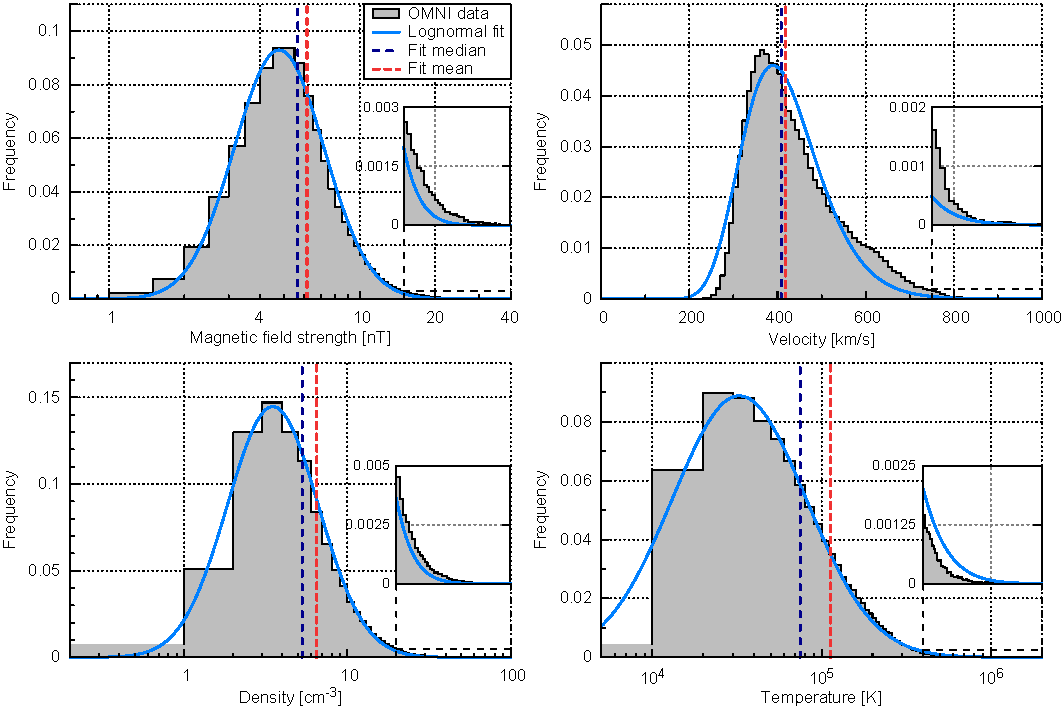
\includegraphics[width=18cm]{figures/histogram_fits_4_a_zoom_paper_pdfplot.pdf}
	\caption{Frequency distributions of the four solar wind parameters and their lognormal fits. The histograms have bins of 0.5~nT, 10~km/s, 1~cm$^{-3}$ and 10\,000~K and are based on the hourly OMNI data set. The fit's median and mean values are indicated as well. The insets only have zoomed-in frequency axes, their x-axes stay the same.}
	\label{fig:histogram_fits_4_a_zoom_paper_pdfplot}
\end{figure*}

%double lognormal fitting
%%%%%%%%%%%%%%%%%%%%%%%%%
%justification for compositional lognormal fit
In order to find a better fit result for the velocity distribution we assume that the velocity distribution can be made up of at least two overlapping branches \citep{McGregor2011b}. Therefore a compositional approach  is chosen by combining two lognormal functions (\ref{eq:single_lognormal_fit_function}), involving more fit variables:
\begin{align}
	W_\text{II}(x) &= c \cdot W_1(x) + (1 -c) \cdot W_2(x)\,.	\label{eq:double_lognormal_fit_function}
\end{align}
The balancing parameter $c$ ensures that the resulting function remains normalized as it represents a probability distribution.

The fitting of $W_\text{II}(x)$ to the velocity's frequency distribution yields the values of the now five fit parameters ($c$, $x_\text{med,1}$, $x_\text{avg,1}$, $x_\text{med,2}$ and $x_\text{avg,2}$) as listed in Table~\ref{tab:lognormal_fit_parameters} together with the median and mean values of the composed distribution, which can be derived via solving
\begin{align}
	\int W_\text{II}(x)\,\text{d}x = 0	&	&\text{and}	&	&\int x\,W_\text{II}(x)\,\text{d}x = 0	\,.
\end{align}
\hl{XXXXXXXXXXXXXXXXXXXXX}\\
As anticipated, this more complex fit function is more accurate in describing the velocity's frequency distribution (see Fig.~\ref{fig:histogram_fits_V_a_zoom_dbl_paper_pdfplot}).
\begin{figure}
	\resizebox{\hsize}{!}{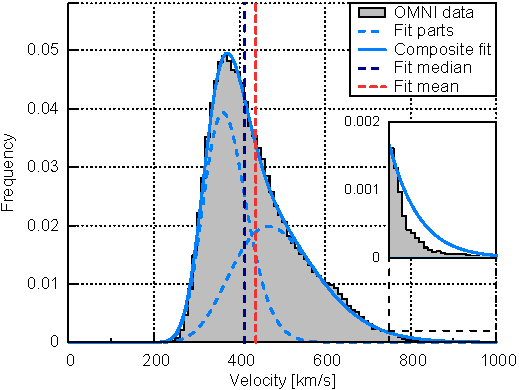
\includegraphics{figures/histogram_fits_V_a_zoom_dbl_paper_pdfplot.pdf}}
	\caption{The velocity's frequency distribution (same as in Fig.~\ref{fig:histogram_fits_4_a_zoom_paper_pdfplot}) and its compositional lognormal fit. The fit's median and mean values and its two fit parts are indicated as well. The inset only has a zoomed-in frequency axis, its x-axis stays the same.}
	\label{fig:histogram_fits_V_a_zoom_dbl_paper_pdfplot}
\end{figure}
For this reason we keep using the double lognormal ansatz for the velocity frequency fits in the following sections.\\
In this static model the slow and fast part contribute almost equally ($c \approx 0.5$), which of course is only valid for this kind of long-term average. At different times in a solar cycle their contributions vary strongly.

%transition
For the bulk of the solar wind these static lognormal functions describe the parameters' distributions well. This is different for the extreme values (which may also stem from CMEs). The simple lognormal fit models of the magnetic field strength, the velocity and the density underestimate their frequency at the high value tails, whereas the temperature's tail is overestimated (see insets of Fig.~\ref{fig:histogram_fits_4_a_zoom_paper_pdfplot}). The velocity's compositional lognormal fit only slightly overestimates its tail (inset in Fig.~\ref{fig:histogram_fits_V_a_zoom_dbl_paper_pdfplot}).

Short-term variations in the solar wind cannot be predicted, but their occurrence rate can. It depends on solar activity, which changes cyclically and thus can be forecasted to a certain degree---at least within a solar cycle.


\section{Solar activity variations}
\label{sec:solar_activity_variations}
This section aims to relate changes in the four solar wind parameters to general solar activity. For this we examine their correlations to the yearly sunspot number and determine the lag times with the highest coefficients. Next, we fit lognormal functions to the frequency distributions like before, but implement linear relations to the yearly SSN to shift the distributions. Only for the velocity the approach is different in that its two components are kept fixed and instead their balance is modified with changing SSN.

\subsection{SSN data}
Solar activity is commonly measured via the sunspot number. We want to correlate OMNI in situ measurements with the SSN, yet OMNI data are from Earth orbit, causing variations in solar latitude and distance. To dodge these seasonal variations we use yearly OMNI and SSN data.

The international sunspot number (\citeyear{sidc}) is retrieved from the online catalogue\footnote{\url{http://www.sidc.be/silso/}} at the World Data Center -- Sunspot Index and Long-term Solar Observations (WDC-SILSO), Solar Influences Data Analysis Center (SIDC), Royal Observatory of Belgium (ROB).

%seasonal influence contained within yearly frequency distributions\\

\subsection{SSN correlation}
Our current interest lies in the correlation of the SSN to the solar wind median values, because the median defines the position of a lognormal function. The yearly OMNI parameter medians and the yearly SSN are plotted in Fig.~\ref{fig:OMNI_yearly_ssn_correlation_c_plot}.

%solar activity = SSN $\neq$ solar cycle\\
The solar wind velocity and its close friends density and temperature are known to depend on the state of the solar cycle \citep{Schwenn1983}, which is why they follow the SSN indirectly (with time lag).
%density modulation with SSN \citep{Schwenn1983} p.~499\\
Thus we derive the correlation coefficients for different time lags between solar wind parameters and SSN (see Fig.~\ref{fig:OMNI_yearly_ssn_correlation_c_plot}).
\begin{figure}
	\resizebox{\hsize}{!}{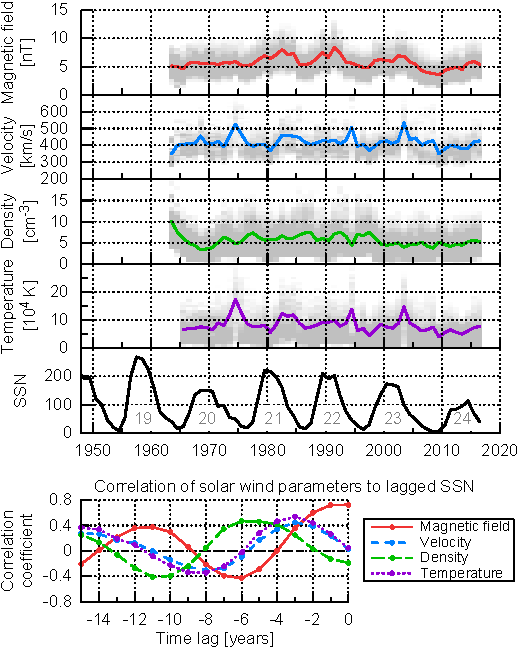
\includegraphics{figures/OMNI_yearly_ssn_correlation_c_plot.pdf}}
	\caption{The solar wind parameter yearly medians from OMNI data and the yearly SSN from the \citet{sidc} with cycle number (top). Their correlation coefficients with the yearly SSN are calculated for time lags back to -15 years (bottom).}
	\label{fig:OMNI_yearly_ssn_correlation_c_plot}
\end{figure}

The highest correlation coefficient for the magnetic field strength is 0.728, which is without lag time and the highest of all solar wind parameters. This is anticipated because the SSN is directly proportional to the magnetic flux \citep{Smith2003}.\\
Velocity and temperature have a lag time of 3~years with their maximal correlation coefficients (0.453 and 0.540). The density has a lag time of 6~years (0.468), which is in agreement with the by \citet{Bougeret1984} documented density anticorrelation with SSN.	%p.~406\\

% maximal correlation coefficients and their lag times:\\
% magnetic field strength: lag 0, 0.728\\
% velocity: lag -3, 0.453\\
% density: lag -6, 0.468\\
% temperature: lag -3, 0.540\\
As expected, the correlation coefficients' amplitudes of all parameters decline with increasing lag time and show a frequency of about 11~years.

\subsection{SSN fitting}
\label{sec:ssn_fitting}
To be able to shift the frequency distributions with SSN, we add a linear SSN dependency to the median
\begin{align}
	x_\text{med}(ssn) &= a_\text{med} \cdot ssn + b_\text{med}\,,	\label{eq:median_with_ssn}
\end{align}
using a factor to the SSN $a_\text{med}$ with a baseline $b_\text{med}$. We relate the mean with a scaling factor to the median to transfer its SSN dependency:
\begin{align}
	x_\text{avg}(ssn) &= (1 + a_\text{avg}) \cdot x_\text{med}(ssn)\,.	\label{eq:mean_with_ssn}
\end{align}
With the implementation of these relations into the lognormal function (\ref{eq:single_lognormal_fit_function}), the new dynamic fit function $W'(x,ssn)$ is then fitted to the yearly data. The three resulting fit coefficients ($a_\text{med}, b_\text{med}$ and $a_\text{avg}$) are presented in Table~\ref{tab:ssn_fit_parameters}.
\begin{table*}
	\caption{Resulting fit coefficients from the OMNI data fitting with lagged SSN. For the velocity the fit parameters from the double lognormal fit and their balancing function are given. The values in brackets are the estimated standard deviation of each fit parameter.}
	\label{tab:ssn_fit_parameters}
	\centering
	\begin{tabular}{l@{} c@{}
		S[table-format = 1.3(2)e+1]
		S[table-format = 1.4(2)]
		S[table-format = 1.3(2)e+1]
		S[table-format = +1.3(2)e+1]
		c
		}
		\hline\hline
		\multicolumn{2}{l}{\multirow{2}{*}{Parameter}}	&\multicolumn{2}{c}{Median\tablefootmark{a}}	&\multicolumn{1}{c}{Mean\tablefootmark{a}}	&\multicolumn{2}{c}{Balance}\\
		\cline{3-4}\cline{6-7}
		\multicolumn{2}{l}{}	&\multicolumn{1}{c}{SSN factor $a_\text{med}$}	&\multicolumn{1}{c}{Baseline $b_\text{med}$}	&\multicolumn{1}{c}{Scaling factor $a_\text{avg}$}	&\multicolumn{1}{c}{SSN factor $c_a$}	&\multicolumn{1}{c}{Baseline $c_b$}\\
		\hline
		\multicolumn{2}{l}{Magnetic field}	&1.309(19)e-2	&4.285(17)	&8.786(78)e-2	&\multicolumn{1}{c}{--}	&--\\
%		\multicolumn{2}{l}{Velocity}	&2.514(93)e-3	&3.8521(90)	&2.392(26)e-2	&\multicolumn{1}{c}{--}	&--\\
		\multicolumn{2}{l}{Density}	&3.81(25)e-3	&4.495(26)	&3.050(27)e-1	&\multicolumn{1}{c}{--}	&--\\
		\multicolumn{2}{l}{Temperature}	&1.974(26)e-2	&5.729(19)	&6.541(28)e-1	&\multicolumn{1}{c}{--}	&--\\
		\hline
		\multirow{2}{*}{Velocity}	&\multicolumn{1}{c}{$W'_1$}	&\multicolumn{1}{c}{--}	&3.633(12)	&1.008(37)e-2	&\multirow{2}{*}{\tablenum{-1.799(95)e-3}}	&\multirow{2}{*}{0.638(32)}\\
			&\multicolumn{1}{c}{$W'_2$}	&\multicolumn{1}{c}{--}	&4.831(81)	&2.31(20)e-2	&	&\\
		\hline
	\end{tabular}
	\tablefoot{
		\tablefoottext{a}{Values in their respective units \si{nT}, \SI{e2}{\km\per\s}, \si{\per\cm\cubed} and \SI{e4}{\K}.}
	}
\end{table*}

Naturally, the fit models match with the general data trends, though single year variations are not able to be replicated by the model (e.g. the high velocity and temperature values in 1974, 1994 and 2003) (see Fig.~\ref{fig:OMNI_yearly_BVdblNTSSN_fit_e_plot}).
\begin{figure*}
	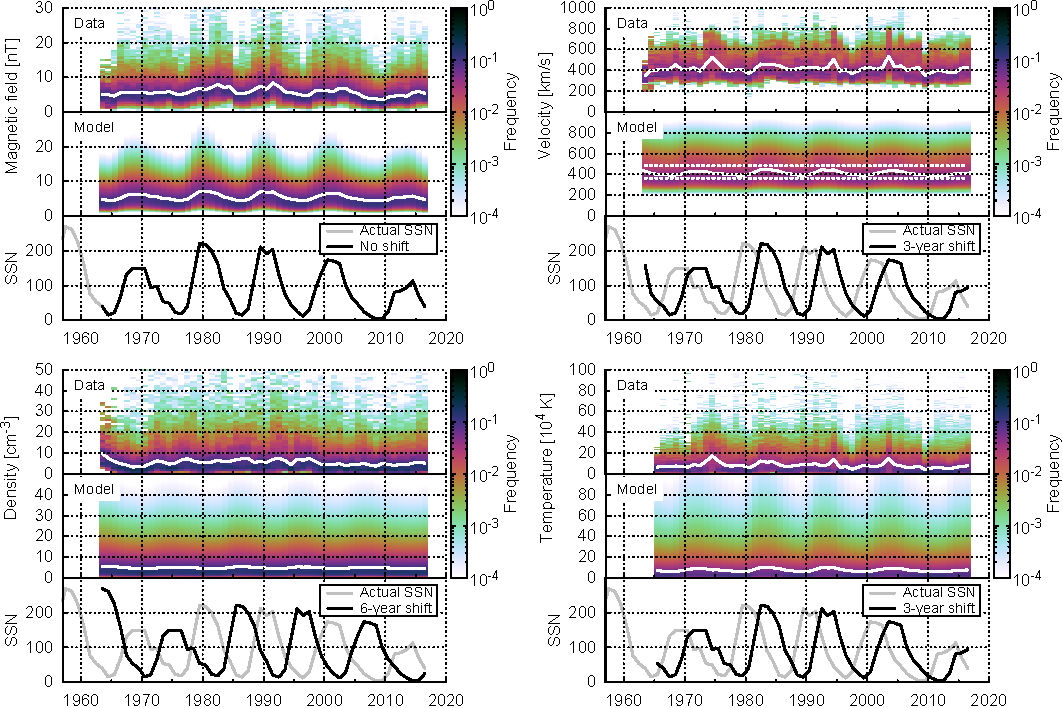
\includegraphics[width=18cm]{figures/OMNI_yearly_BVdblNTSSN_fit_e_plot.pdf}
	\caption{Solar wind parameter data frequencies, lognormal fit models with their median values (white) and the corresponding yearly SSN (grey) over the OMNI time period 1963--2016. The for the models shifted SSN is indicated by a black line. The velocity median is derived from the SSN weighted constant lognormal parts (dotted).}
	\label{fig:OMNI_yearly_BVdblNTSSN_fit_e_plot}
\end{figure*}
The comparison with the yearly data median values over SSN shows that the from the model obtained medians have a quite similar slope (see Fig.~\ref{fig:OMNI_yearly_BVNTvsSSN_a}).
\begin{figure}
	\resizebox{\hsize}{!}{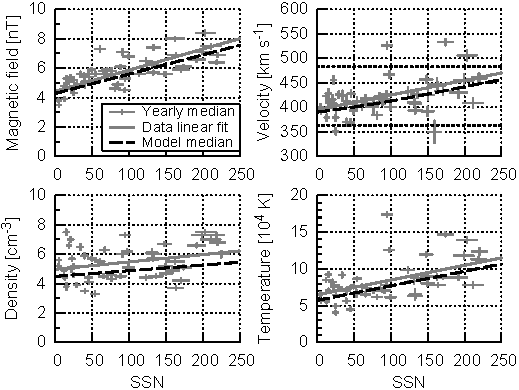
\includegraphics{figures/OMNI_yearly_BVNTvsSSN_a.pdf}}
	\caption{Solar wind parameter median over lagged SSN. The yearly data medians (+) with their weighted linear fit (solid) are obtained from OMNI data. The error bars denote the SSN standard deviation and the relative weight from the yearly data coverage. The SSN dependent median (\ref{eq:median_with_ssn}) is from the lognormal model fit (dashed). For the velocity the median is derived from the SSN weighting of the slow and fast model parts, whose magnitudes are SSN independent (dotted).}
	\label{fig:OMNI_yearly_BVNTvsSSN_a}
\end{figure}

Again, the velocity gets a special treatment with the double lognormal distribution (\ref{eq:double_lognormal_fit_function}). It is known that slow and fast solar wind stream occurrence rates follow the solar cycle, yet their magnitudes stay fairly stable (cite?). Thus we keep the two velocity components' positions constant and vary instead their balance with the SSN:
\begin{align}
	c(ssn) &= c_a \cdot ssn + c_b\,.	\label{eq:balance_with_ssn}
\end{align}
The fit result (see Table~\ref{tab:ssn_fit_parameters}) is a model in which three years after solar cycle minimum (SSN of zero) the slow solar wind has a share of almost two-thirds and decreases further with increasing SSN (see Fig.~\ref{fig:Vdbl_SSN_ratio_f_plot}).\\
\begin{figure}
	\resizebox{\hsize}{!}{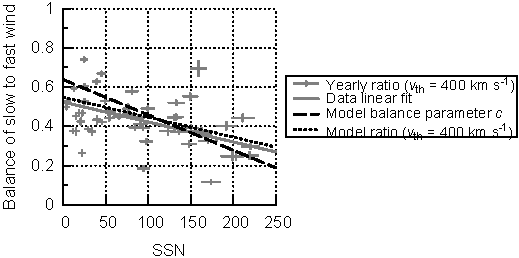
\includegraphics{figures/Vdbl_SSN_ratio_f_plot.pdf}}
	\caption{Balance of slow to fast solar wind over the by 3~years lagged SSN. The yearly ratios (+) and their weighted linear fit (solid) are obtained from OMNI data with a threshold velocity of $v_\text{th} = \SI{400}{\km\per\s}$. The error bars denote the SSN standard deviation and the relative weight from the yearly data coverage. The model's balance parameter (\ref{eq:balance_with_ssn}) and derived ratio (same threshold) are plotted as dashed and dotted lines.}
	\label{fig:Vdbl_SSN_ratio_f_plot}
\end{figure}
% 3 years after minimum (SSN of zero) the slow wind has its maximal share of 0.638(32). 3 years after maximum (SSN of 200) it has only a share of 0.278(37).\\
To compare the ratios of slow to fast wind between model and data, we simply apply the commonly used constant velocity threshold of $v_\text{th} = \SI{400}{\km\per\s}$ (cite?). The linear fit to the yearly data ratio and the derived model ratio are quite similar (see Fig.~\ref{fig:Vdbl_SSN_ratio_f_plot}). Specific velocity thresholds between slow and fast solar wind cannot be directly compared with the to some degree steeper balance parameter of this model. The model's balance may represent the actual ratios of the solar wind types in a more realistic way than a specific velocity threshold does, since the velocity ranges of both types overlap \citep{McGregor2011b}.
%(i.e. there exists slow wind with properties of fast wind and vice versa)


%exponential fitting
%%%%%%%%%%%%%%%%%%%%
\section{Solar distance dependency}
\label{sec:solar_distance_dependency}
In this section we use Helios data to obtain power law fit functions for the heliocentric distance dependency and also evaluate the fits' extrapolation behavior in direction to the Sun. To fit the bulk solar wind distributions' distance dependency we use the frequency fitting method from Sect.~\ref{sec:frequency_distribution} on distance-binned Helios data. This results in models comprising of with distance shifted lognormal functions.

%Helios data
\subsection{Helios distance data}
\label{sec:helios_distance_data}
The Helios probes were the only spacecraft measuring in situ solar wind over large solar distance ranges in the inner heliosphere. We use the combined data from both Helios~1 and Helios~2 probes. Helios~1's (Helios~2's) highly elliptical orbit in the ecliptic covered a solar distance range of \SIrange{0.31}{0.98}{\au} (\SIrange{0.29}{0.98}{\au}). Launched during solar cycle minimum, the data of both probes cover the rise to the maximum of cycle 21 ($\sim$6.5~years at varying distances).

%hourly data
Again we choose data with hourly resolution to allow its use along with the hourly OMNI data. As \citet{Schwenn1983} pointed out, the many hourly Helios data points which contain only a few measurements, contribute with a larger scatter to the frequency distributions, nevertheless their effect is insignificant in the treatment of the bulk data.	%\citet[p.~491]{Schwenn1983} 

Helios~1's (Helios~2's) merged hourly data set from the magnetometer and plasma instruments \citep{Rosenbauer1977} includes $\sim$12.5~orbits ($\sim$8~orbits) in the time range \mbox{1974-12-10} to \mbox{1981-06-14} (\mbox{1976-01-01} to \mbox{1980-03-04}).
%Helios plasma instrument (E1); Helios magnetometer instrument (E2)
% Helios data ranges:\\
% - time range Helios~1 [1974-12-10--1981-06-14] (12.5~orbits), Helios~2 [1976-01-01--1980-03-04] (8~orbits)\\
% - solar distance range Helios~1 0.31--0.98~au, Helios~2 0.29--0.98~au\\
%data sources
The Helios data was retrieved from the Coordinated~Data~Analysis~Web (CDAWeb) interface at NASA's GSFC/SPDF\footnote{\url{http://spdf.gsfc.nasa.gov/}}.

The Helios~1 (Helios~2) magnetometer data coverage is about 43~\% (54~\%) and amounts to 2.8~years (2.3~years) in total. The plasma data coverage is 76~\% (92~\%) and amounts to 5.0~years (3.9~years) in total.
% temporal coverage of merged data\\
% Helios 1: 1974-12-10--1981-06-14; 6y6m15d = 2388~d = 6.538~y\\
% Mag data coverage: 42.6~\%; 2.785~years\\
% Plasma data coverage: 76.4~\%; 4.995~years\\
% Helios 2: 1976-01-01--1980-03-04; 4y3m4d = 1557~d = 4.263~y\\
% Mag data coverage: 54.4~\%; 2.319~years (83~\% of H1)\\
% Plasma data coverage: 91.8~\%; 3.913~years (78~\% of H1)\\
Thus, the Helios data cover only fractions of a solar cycle and cannot be used for deriving representative time-independent solar wind multi-cycle conditions like the OMNI data can.

%Helios data biased towards solar minimum
Using this data, we also have to keep in mind that its time coverage is unequally distributed over the solar cycle. Dividing the data by the transition from cycle minimum to maximum (mid 1977) and considering the data gap distributions, the Helios data covers about \SI{68}{\percent} during cycle minimum whereas during maximum only \SI{38}{\percent}.

% data gaps -> uneven coverage -> solar cycle minimum dominates; ratio of max vs min cycle data coverage; for OMNI data negligible\\
% 13~months smoothed sunspot number \citep{sidc}: divide June~1977 (include figure)\\
% put link on sidc webpage: http://sidc.be/sunspot-data/SIDCpub.php
% begin: 1974-12 36.1\\
% minimum: May/June 1976 18.3/17.9 (cite?)\\
% divide 30~June~1977 37.7 from SIDC data (nearly same SSN as at Helios~1 beginning)\\
% cycle 21 maximum: Dec 1979 232.9 (cite?)\\
% end: 1981-06 200.9\\
% 
% data gap hours and percentages:\\
% % H1 minimum 22416 h\\
% % H1 maximum 34681 h\\
% % H2 minimum 13128 h\\
% % H2 maximum 23472 h\\
% % sum 93697 h\\
% solar minimum: 35\,544~h, 37.94~\%\\
% solar maximum: 58\,153~h, 62.06~\%\\

% 1974 11 1974.874   39.3   4.2    30  
% 1974 12 1974.958   36.1   4.0    31  
% 1975 01 1975.042   33.0   3.9    31  
% 1975 02 1975.123   31.8   3.8    28  
% 1975 03 1975.204   30.6   3.7    31  
% 1975 04 1975.288   26.8   3.5    30  
% 1975 05 1975.371   24.2   3.3    31  
% 1975 06 1975.455   23.2   3.3    30  
% 1975 07 1975.538   21.8   3.2    31  
% 1975 08 1975.623   20.7   3.1    31  
% 1975 09 1975.707   20.9   3.1    30  
% 1975 10 1975.790   22.3   3.2    31  
% 1975 11 1975.874   23.3   3.3    30  
% 1975 12 1975.958   23.6   3.3    31  
% 1976 01 1976.042   22.1   3.2    31  
% 1976 02 1976.124   19.2   3.0    29  
% 1976 03 1976.206   17.8   2.9    31  
% 1976 04 1976.290   18.4   2.9    30  
% 1976 05 1976.373   18.3   2.9    31  
% 1976 06 1976.456   17.9   2.9    30  
% 1976 07 1976.540   18.8   2.9    31  
% 1976 08 1976.624   20.5   3.1    31  
% 1976 09 1976.708   20.8   3.1    30  
% 1976 10 1976.791   19.7   3.0    31  
% 1976 11 1976.874   19.7   3.0    30  
% 1976 12 1976.958   21.6   3.2    31  
% 1977 01 1977.042   24.3   3.3    31  
% 1977 02 1977.123   26.3   3.5    28  
% 1977 03 1977.204   28.8   3.6    31  
% 1977 04 1977.288   31.9   3.8    30  
% 1977 05 1977.371   34.7   4.0    31  
% 1977 06 1977.455   37.7   4.1    30  
% 1977 07 1977.538   41.4   4.3    31  
% 1977 08 1977.623   47.6   4.6    31  
% 1977 09 1977.707   55.8   5.0    30  
% 1977 10 1977.790   64.8   5.4    31  
% 1977 11 1977.874   73.7   5.7    30  
% 1977 12 1977.958   80.7   6.0    31  
% 1978 01 1978.042   86.9   6.2    31  
% 1978 02 1978.123   91.5   6.4    28  
% 1978 03 1978.204   98.7   6.6    31  
% 1978 04 1978.288  109.0   7.0    30  
% 1978 05 1978.371  117.8   7.2    31  
% 1978 06 1978.455  126.6   7.5    30  
% 1978 07 1978.538  138.0   7.8    31  
% 1978 08 1978.623  147.3   8.1    31  
% 1978 09 1978.707  153.6   8.3    30  
% 1978 10 1978.790  157.3   8.4    31  
% 1978 11 1978.874  160.4   8.5    30  
% 1978 12 1978.958  166.7   8.6    31  
% 1979 01 1979.042  175.2   8.8    31  
% 1979 02 1979.123  185.4   9.1    28  
% 1979 03 1979.204  193.3   9.3    31  
% 1979 04 1979.288  199.9   9.4    30  
% 1979 05 1979.371  208.5   9.6    31  
% 1979 06 1979.455  216.7   9.8    30  
% 1979 07 1979.538  219.5   9.9    31  
% 1979 08 1979.623  220.1   9.9    31  
% 1979 09 1979.707  220.4   9.9    30  
% 1979 10 1979.790  223.4  10.0    31  
% 1979 11 1979.874  229.8  10.1    30  
% 1979 12 1979.958  232.9  10.2    31  
% 1980 01 1980.042  232.0  10.2    31  
% 1980 02 1980.124  230.2  10.2    29  
% 1980 03 1980.206  227.9  10.1    31  
% 1980 04 1980.290  224.6  10.0    30  
% 1980 05 1980.373  221.3  10.0    31  
% 1980 06 1980.456  219.1   9.9    30  
% 1980 07 1980.540  216.1   9.9    31  
% 1980 08 1980.624  212.0  10.0    31  
% 1980 09 1980.708  211.5  10.2    30  
% 1980 10 1980.791  211.9  10.5    31  
% 1980 11 1980.874  209.1  10.9    30  
% 1980 12 1980.958  202.8  11.0    31  
% 1981 01 1981.042  199.6  11.1   271  
% 1981 02 1981.123  202.2  11.5   229  
% 1981 03 1981.204  205.4  12.1   244  
% 1981 04 1981.288  205.7  12.6   254  
% 1981 05 1981.371  204.1  12.8   268  
% 1981 06 1981.455  200.9  13.1   227  
% 1981 07 1981.538  198.5  13.1   268  

For calculating the median and mean values at different solar distances the data is binned into \SI{0.01}{\au} bins, which is also the native precision in this data set.

\subsection{Power law fitting}
\label{sec:power_law_fitting}
%why power law function?
A power law scaling distance behavior is expected from all four parameters (cites?). Therefore we use the power function
\begin{align}
	x(r) = d\,r^e	\label{eq:power_function}
\end{align}
with the solar distance $r$ for the regression fit of the median and mean. The fits are weighted by data counts per bin.
%fit result table and figure
With $r$ in astronomical units we get the fit coefficients ($d_\text{med}$, $d_\text{avg}$, $e_\text{med}$ and $e_\text{avg}$) as given in Table~\ref{tab:mean_median_fit_parameter}.
\begin{table*}
	\caption{Fit coefficients for the median and mean solar distance dependencies of the four parameters from the combined Helios data set. The errors in brackets are the estimated standard deviations of each fit parameter. The crossing distance is the point where the fitted median and mean intersect. The year variation is the weighted standard deviation from all yearly fitted exponents.}
	\label{tab:mean_median_fit_parameter}
	\centering
	\begin{tabular}{l
	S[table-format = 1.3(2)]
	S[table-format = +1.3(2)]
	@{}c
	S[table-format = 1.3(2)]
	S[table-format = +1.3(2)]
	S[table-format = 1.1(2)e1]
	S[table-format = 1.3]}
		\hline\hline
		\multirow{2}{*}{Parameter}	&\multicolumn{2}{c}{Median}	&	&\multicolumn{2}{c}{Mean}	&\multicolumn{1}{c}{Crossing distance}	&\multicolumn{1}{c}{Year variation}\\
		\cline{2-3}	\cline{5-6}
			&\multicolumn{1}{c}{$d_\text{med}$\tablefootmark{a}}	&\multicolumn{1}{c}{$e_\text{med}$}	&	&\multicolumn{1}{c}{$d_\text{avg}$\tablefootmark{a}}	&\multicolumn{1}{c}{$e_\text{avg}$}	&\multicolumn{1}{c}{[\si{\au}]}	&\multicolumn{1}{c}{$\Delta e$}\\
		\hline
		Magnetic field	&5.377(92)	&-1.655(17)	&	&6.05(10)	&-1.546(18)	&0.339(11)	&0.11\\
		Velocity	&4.107(28)	&0.058(13)	&	&4.356(24)	&0.049(10)	&0.7(83)e3	&0.012\\
		Density		&5.61(27)	&-2.093(46)	&	&7.57(30)	&-2.010(38)	&0.027(73)	&0.072\\
		Temperature	&7.14(23)	&-0.913(39)	&	&9.67(21)	&-0.792(28)	&0.082(85)	&0.005\\
		\hline
	\end{tabular}
	\tablefoot{
		\tablefoottext{a}{Values in their respective units \si{nT}, \SI{e2}{\km\per\s}, \si{\per\cm\cubed} and \SI{e4}{\K}.}
	}
\end{table*}
% source year variation: fit_out_yearly_gradients_table_b_stats.txt

% comparison with other Helios studies (Schwenn, Bougeret)
As expected, the velocity exponents match with those from \citet{Schwenn1983,Schwenn1990}, who derived the distance dependencies for both Helios spacecraft separately ($v_\text{H1}(r) \propto r^{0.083}$ and $v_\text{H2}(r) \propto r^{0.036}$).
%Helios results, radial gradients see \citet{Schwenn1990} p.~155\\
Likewise, the density exponents agree well with the Helios plasma density model, which \citet{Bougeret1984} derived from Helios data and normed to the 1976 \SI{1}{\au} density ($n(r) = 6.14\,r^{-2.10}\,\text{cm}^{-3}$).

%crossing distances
The next step is to fit the bulk of the solar wind parameters with lognormal functions. At all considered solar distances the mean of the three plasma parameters is larger than their median (Fig.~\ref{fig:radial_fit_4_thesis_light_skip_pdfcairo_plot}).
\begin{figure*}
	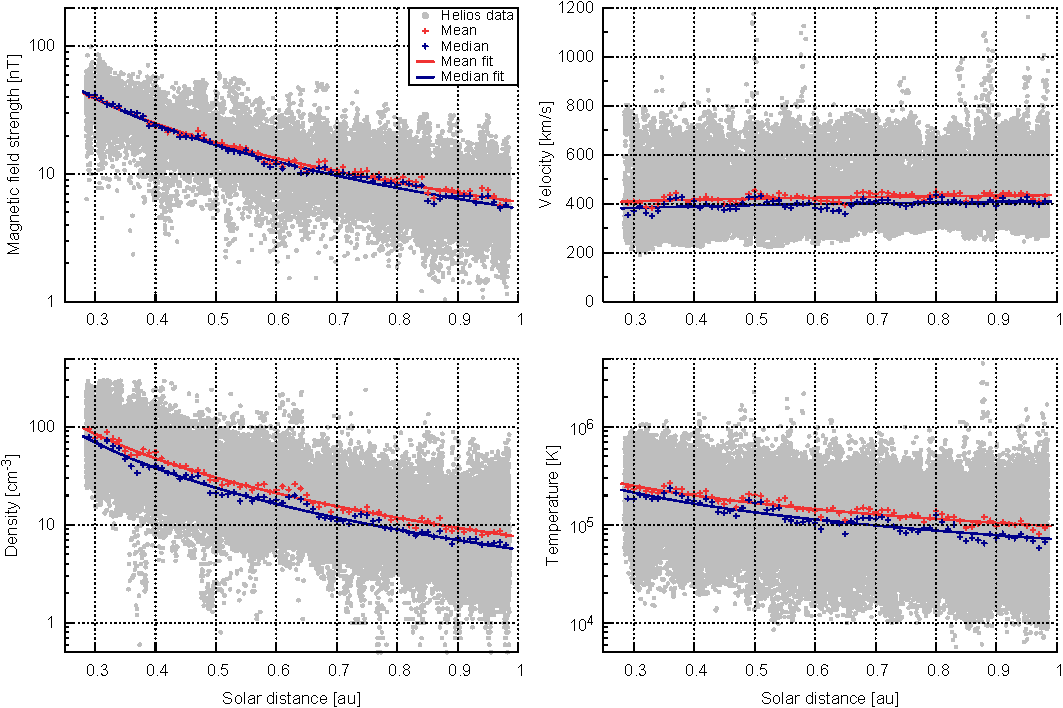
\includegraphics[width=18cm]{figures/radial_fit_4_thesis_light_skip_pdfcairo_plot.pdf}
	\caption{Helios hourly data plots of the four solar wind parameters over solar distance. The mean and median per \SI{0.01}{\au} data bin and their fit curves are plotted as well. The Helios data has a native distance resolution of \SI{0.01}{\au}. To make the abundance visible in these plots, we added a random distance value of up to \SI{+-0.005}{\au}.}
	\label{fig:radial_fit_4_thesis_light_skip_pdfcairo_plot}
\end{figure*}

The large velocity's crossing distance and its large error indicate that the median's and mean's distance behavior can be kept identical and so the frequency's shape distance independent.

However, the magnetic field strength's mean crosses the median at \SI{0.339}{\au} and is lower at smaller distances (Table~\ref{tab:mean_median_fit_parameter}). At the crossing point and below the magnetic field strength can therefore not be described anymore with a lognormal function. For an extrapolation to the PSP perihelion the same happens for the temperature at \SI{0.082}{\au}.

Those crossings limit the possible extrapolation distances with lognormal functions. To circumvent these limitations for all four solar wind parameters we set the exponents $e_\text{med}$ and $e_\text{avg}$ to be identical, avoiding crossing of median and mean. Then the distribution's width has a power law scaling with solar distance. Applying this approximation, we have to accept larger model errors, especially for the magnetic field strength. It also limits the extrapolation accuracy, however it keeps the model simpler.

\subsection{Power law lognormal fitting}
To retrieve the frequency distributions for every \SI{0.01}{\au} solar distance bin, we choose the same solar wind parameter binning as with the OMNI data (Sect.~\ref{sec:frequency_distribution}).
% Helios histogram bin sizes for mean of frequency distribution (at specific solar distance):\\
% $B$: bin size 0.5~nT, min 337, mean precision: 0.000545\\
% $v$: bin size 1~cm$^{-3}$, min 497, mean precision: 0.00449\\
% $n$: bin size 10~km/s, min 497, mean precision:  0.00449\\
% $T$: bin size 10\,000~K, min 497, mean precision: 4.49--44.49\\

As mentioned before, we set the exponents of median and average to be identical. Implementing the power law distance dependency~(\ref{eq:power_function}) into the lognormal function (\ref{eq:single_lognormal_fit_function}), we get three fit parameters ($d'_\text{med}$, $d'_\text{avg}$ and the common exponent $e'$). Naturally, we use the double lognormal function~(\ref{eq:double_lognormal_fit_function}) for the velocity distribution fit, resulting in $W''_\text{II}(x,r)$. The additional fit parameters are the balancing parameter $c'$ and from the second lognormal part $d'_\text{med,2}$ and $d'_\text{avg,2}$. The resulting fit coefficients for the four solar wind parameters are presented in Table~\ref{tab:extrapolation_model_fit_parameters}.
\begin{table*}
	\caption{Fit coefficients from the single lognormal power function, respectively double lognormal for the velocity (combined Helios data). The errors in brackets are the estimated standard deviations of each fit parameter.}
	\label{tab:extrapolation_model_fit_parameters}
	\centering
	\sisetup{table-figures-integer=1, table-figures-decimal=3, table-figures-exponent=0}
	\begin{tabular}{l c
	S[table-format = 1.3(2), table-space-text-post = a, table-align-text-post = false]
	S[table-format = 1.3(2), table-space-text-post = a, table-align-text-post = false]
	S[table-format = +1.4(2)]
	S[table-format = 1.3(2)]}
		\hline\hline
		\multicolumn{2}{l}{\multirow{2}{*}{Parameter}}	&\multicolumn{1}{c}{Median\tablefootmark{a}}	&\multicolumn{1}{c}{Mean\tablefootmark{a}}	&\multicolumn{1}{c}{Exponent}	&\multicolumn{1}{c}{Balance}\\
			&	&\multicolumn{1}{c}{$d'_\text{med}$}	&\multicolumn{1}{c}{$d'_\text{avg}$}	&\multicolumn{1}{c}{$e'$}	&$c'$\\
		\hline
		\multicolumn{2}{l}{Magnetic field}	&5.358(25)	&5.705(28)	&-1.662(11)	&\multicolumn{1}{c}{--}\\
		\multicolumn{2}{l}{Density}	&5.424(33)	&6.845(47)	&-2.114(20)	&\multicolumn{1}{c}{--}\\
		\multicolumn{2}{l}{Temperature}	&6.357(64)	&10.72(14)	&-1.100(20)	&\multicolumn{1}{c}{--}\\
		\hline
		\multirow{1}{*}{Velocity}	&$W''_1$	&3.707(13)	&3.748(16)	&\multirow{2}{*}{0.0990(51)}	&\multirow{2}{*}{0.557(45)}\\
			&$W''_2$	&5.26(13)	&5.42(11)	&	&\\
		\cline{2-6}
		\multicolumn{2}{r}{$W''_\text{II}$}	&4.13(13)\tablefootmark{b}	&4.47(11)\tablefootmark{b}	&\multicolumn{1}{c}{--}	&\multicolumn{1}{c}{--}\\
		\hline
	\end{tabular}
	\tablefoot{
		\tablefoottext{a}{Values in their respective units \si{nT}, \SI{e2}{\km\per\s}, \si{\per\cm\cubed} and \SI{e4}{\K}.}
		\tablefoottext{b}{Velocity median and mean \SI{1}{\au} values for the resulting function. Error estimates derived from the individual fit part errors.}
	}
\end{table*}
% Vdbl fit:
% medians = 370.7, 526
% means = 374.8, 542
% c = 0.557
% via calculate_twolognormal_median.py:
% mean = 446.64
% median = 413.33

With $c' = 0.557$ the velocity balancing parameter is of an expected value similar to that obtained from the Helios time period (the mean SSN during the Helios period was 59, this corresponds to $c(59) = 0.53$; see Fig.~\ref{fig:Vdbl_SSN_ratio_f_plot}).

The fit models seem to resemble the data quite well (Fig.~\ref{fig:mixed_fit_fixed_4_paper_f_plot}). The magnetic field strength frequency is more focused (around \SI{40}{nT}) at the lower distance boundary than the model's is. This is expected because of our fixed distance independent shape approximation.
\begin{figure*}
	\includegraphics[width=18cm]{figures/mixed_fit_fixed_4_paper_f_plot.pdf}
	\caption{Solar wind parameter's frequency distributions over solar distance. Plotted are the binned Helios data and the power law lognormal fit model (double lognormal for the velocity) with their median values (white).}
	\label{fig:mixed_fit_fixed_4_paper_f_plot}
\end{figure*}
The velocity and temperature models' upper values have a higher frequency than the data shows. This is due to the systematic fit discrepancy of the lognormal distribution's high value tails (see zoom box in Fig.~\ref{fig:histogram_fits_4_a_zoom_paper_pdfplot}).

\subsection{Distance scaling law variations}
\label{sec:distance_scaling_law_variations}

relocate section to 5.3?\\

This radial solar wind model represents the Helios time frame around the rise of solar cycle~21. It is known that the solar wind parameters' magnitudes vary with solar activity. Looking at the variation of the yearly distance scaling laws (Fig.~\ref{fig:yearly_gradients_b}), there is no systematic variation for the magnetic field. The exponents of velocity and temperature seem to follow the SSN and the density not...
\begin{figure}
	\resizebox{\hsize}{!}{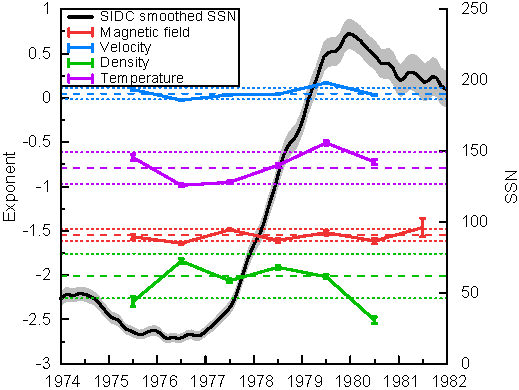
\includegraphics{figures/yearly_gradients_b.pdf}}
	\caption{Helios year variation of the solar wind parameters' fit exponents and SIDC 13-month smoothed monthly SSN. In this plot the year 1974 is omitted because the 21 days covered only }
	\label{fig:yearly_gradients_b}
\end{figure}

For simplicity we assume that the distance scaling laws are time independent and account for this approximation with including the calculated exponents' yearly variations (Table~\ref{tab:mean_median_fit_parameter}) as uncertainities.\\

make remark about influence of unequal solar cycle coverage... (sect.~5.1)\\

Possible differing scaling laws at smaller heliocentric distances are discussed in Sect.~\ref{sec:model_extrapolation_to_psp_orbital_time_and_position}.


\section{General solar wind model}
\label{sec:general_solar_wind_model}

Finally, we combine the obtained solar activity and distance dependencies for shifting the frequency distributions. The result is an empirical solar wind model for the inner heliosphere.\\

%are the exponents time-independent?
Under the assumption that the fall-off laws do not change with time/solar activity (as shown above...), they can be used in general.

We combine the fit coefficients of the median relation for solar activity dependence (\ref{eq:median_with_ssn}) with the ones from the power law distance dependence (previous section)
\begin{align}
	x_\text{med}(ssn,r) &= (a_\text{med} \cdot ssn + b_\text{med}) \cdot r^{e'}
\end{align}

to get the combined model function $W'''(x,ssn,r)$. And for the velocity $W_\text{II}'''(x,ssn,r)$ with the double lognormal function (\ref{eq:double_lognormal_fit_function}).\\

%model errors
%give model errors sizes/uncertainties (sigmas); $W'''_\text{err}(x,ssn,r)$, $x_\text{med\_err}(ssn,r)$\\

% model requirements:\\
% - modeling the frequency distribution with sufficient accuracy -> error size (changing distribution shape with distance)\\
% - modeling the distance dependency with sufficient accuracy -> error size (different scaling law at smaller distances?)\\
% - possibility to extrapolate model down to \SI{0.0459}{\au}\\

%model limits
empirical model limits (spherical coordinates):\\
- heliocentric distance range \SIrange{0.29}{0.98}{\au}\\
- rotational symmetry\\
- confined to ecliptic (\SI{+-7.2}{\degree} HGI)\\
model constrictions:\\
- solar distance dependency function\\
- frequency distribution functions\\
- neglected influence from heliolatitude variation\\


\section{Model extrapolation to PSP orbital time and position}
\label{sec:model_extrapolation_to_psp_orbital_time_and_position}
To estimate the solar wind environment at PSP's planned orbital positions during its mission time, SSN predictions are included into the general solar wind model and extrapolations to the PSP perihelion region are performed.

\subsection{SSN prediction for PSP mission time}
%SSN prediction
For the SSN short-term prediction are several sources available. The SIDC provides 12-month SSN forecasts\footnote{\url{http://sidc.be/silso/forecasts}} obtained from different methods (e.g. Kalman filter combined method). The Space Weather Prediction Center's (SWPC) prediction follows a consensus of the Solar~Cycle~24 Prediction~Panel\footnote{\url{http://www.swpc.noaa.gov/products/solar-cycle-progression}} (until end of 2019).

For the prediction of the next solar cycle~25 we simply assume a course similar to the last and thus we shift the last cycle by 11~years. Additionally we consider the two alternatives of half and twice its amplitude. The SSN for PSP's first perihelion will be small---certainly below 20, whereas its nearest perihelia, which commence at the height of cycle~25, will have as of now almost unpredictable SSN amplitudes (see Fig.~\ref{fig:SPP_orbit_predicted_SSN_overview_e_plot}).
\begin{figure}
	\resizebox{\hsize}{!}{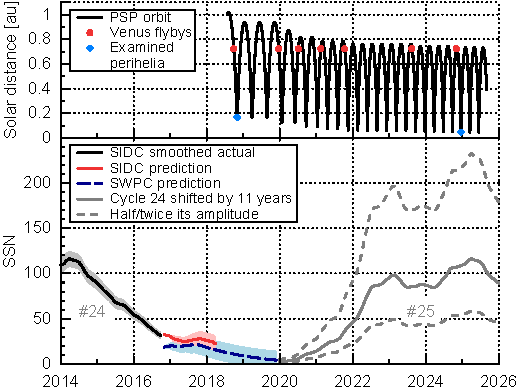
\includegraphics{figures/SPP_orbit_predicted_SSN_overview_e_plot.pdf}}
	\caption{PSP's solar distance during its mission time (top). Consecutive Venus flybys bring its perihelia nearer to the Sun. Actual and predicted SSN (bottom), i.e. SIDC 13-month smoothed monthly actual SSN, SIDC prediction, SWPC prediction and simply by 11~years shifted SSN from previous cycle~24, together with two alternative trends of half and twice its amplitude.}
	\label{fig:SPP_orbit_predicted_SSN_overview_e_plot}
\end{figure}

\subsection{Near-Sun extrapolation for PSP orbit}
%PSP orbit
Parker Solar Probe is planned to launch in mid 2018. With its first Venus flyby it will swing into Venus' orbital plane (\SI{3.86}{\degree} to Sun's equator/\SI{3.39}{\degree} to ecliptic), which allows for additional seven flybys to finally reduce its perihelion distance to a minimum of less than \SI{10}{R_s} \citep{Fox2015} (Fig.~\ref{fig:SPP_orbit_predicted_SSN_overview_e_plot}).\\

For the extrapolation to PSP's orbital range we just assume that our derived distance scaling laws do not change. The comparison with existing near-Sun models reveals that this is not entirely true (Fig.~\ref{fig:sw_extrapolation_ssn_b_plot}).\\
\begin{figure*}
	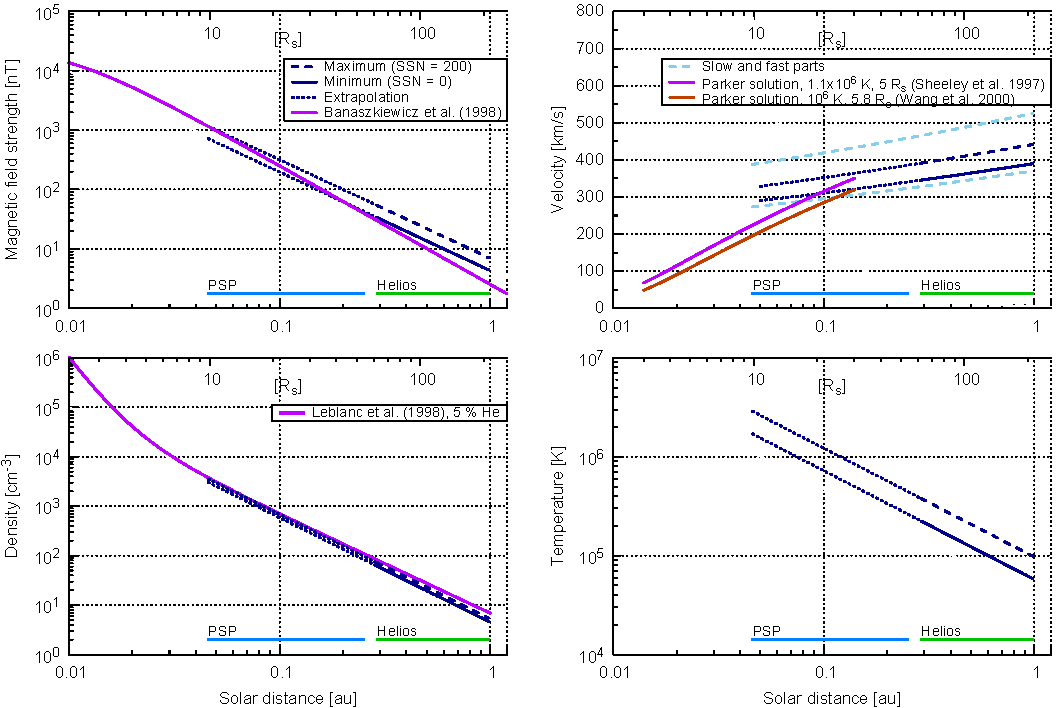
\includegraphics[width=18cm]{figures/sw_extrapolation_ssn_b_plot.pdf}
	\caption{Radial extrapolation of the solar wind parameters to the PSP orbit region. The from Helios and OMNI measurements obtained models are extrapolated to the PSP region---for the extreme cases of solar minimum (SSN = 0) and maximum (SSN = 200). Note that there is a time lag to the SSN depending on the solar wind parameter. The magnetic field radial dependence is slightly flatter than the analytic DQCS model for solar minimum which \citet{Banaszkiewicz1998} derived. Below \SI{20}{R_s} the slow wind velocity is overestimated in comparison to the measurements from \citet{Wang2000}) and \citep{Sheeley1997}. They derived temperature and sonic point values for slow solar wind with the isothermal expansion model \citep{Parker1958}. Down to PSP's perihelion the density is in good agreement with the model from \citet{Leblanc1998}. to 1-column...?}
	\label{fig:sw_extrapolation_ssn_b_plot}
\end{figure*}

%magnetic field:
The magnetic field magnitude from our extrapolation is flatter than the analytical magnetic field model from \citet{Banaszkiewicz1998}, who constructed a dipole plus quadrupole plus current sheet (DQCS) model. We attribute this effect to the from a lognormal shape deviating distribution (see Sect.~\ref{sec:power_law_fitting}).\\

%velocity:
%critical surfaces
Alfvénic critical surface i.e. source surface (see Fox before 2.1)\\
in direction to the Sun is at about \SI{2.5}{R_s} the source surface (Schatten1969)\\
sonic and Alfvénic critical point positions (see \citet{Sittler1999})\\
sonic point and slow solar wind origin \citep{Sheeley1997}\\
approaching these regions, acceleration plays a role\\

\citet{Wang2000}, sources of slow solar wind + IMF regulation mechanism + blobs; compare with our slow V lognormal part; Parker solution\\
-> below 20~Rs PSP will fly well into sw acceleration region\\

\citet{Sheeley1997} -> LASCO coronagraph observed speed profile of coronal features tracing the slow solar wind, 2--30~Rs\\
%- parabolic eq.~(2) and exponential eq.~(3)\\
- sonic point 5--6~Rs\\
- slow solar wind origin 3--4~Rs\\

The near-Sun (PSP perihelion) solar wind velocity is expected to be slower than our model's estimates, because the position of the source (Alfvénic critical) surface is predicted to lie between 15--30~Rs (Schatten1969, Sittler1999, Exarhos2000, Katsikas2010, Goelzer2014; choose references...), up to which the solar wind is believed to be accelerated.\\
The \citet{Parker1958} model of an isothermal expanding corona with a temperature of \SI{e6}{\K} and a critical radius of \SI{5.8}{R_s}.\\

%density:
We expect that even our Sun-nearest extrapolated density at PSP perihelion agrees well with the actual, since \citet{Leblanc1998} derived an electron density model from type~III radio burst observations. Their model shows that the density distance dependency scales with $r^{-2}$ and steepens not until below \SI{10}{R_s} with $r^{-6}$ (see Fig.~\ref{fig:sw_extrapolation_ssn_b_plot}).\\

magnetic field and temperature:\\
crossing distance effect\\

% The model of \citet{Sittler1999} is based on Skylab coronagraph and Ulysses data. it is a 2d semiempirical MHD model (time static)\\
% L-> compare with their radial density function eq. (18a); B-field function eq. (19a+b); V(r) eq. (24); T(r)...\\

\subsection{PSP solar wind environment estimation}
Implementing the orbital distance data and predicted SSN for the mission time we can derive PSP's estimated solar wind environment $W'''(x,ssn,r)$.\\
The zoom into the first and the nearest perihelia show which solar wind parameter magnitudes can be expected there (Figs.~\ref{fig:SPP_perihelia_prediction_e_plot} and \ref{fig:SPP_perihelia_prediction_nearest_e_plot}).\\
\begin{figure}
	\resizebox{\hsize}{!}{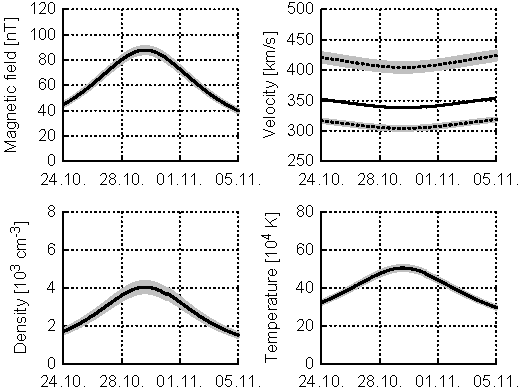
\includegraphics{figures/SPP_perihelia_prediction_e_plot.pdf}}
	\caption{Estimated solar wind parameter medians (black) and their error bands (grey) during 12 days in 2018 with PSP's first perihelion at about \SI{0.16}{\au}. For the velocity the combined median is calculated and also the SSN independent slow and fast parts are plotted (dotted).}
	\label{fig:SPP_perihelia_prediction_e_plot}
\end{figure}
\begin{figure}
	\resizebox{\hsize}{!}{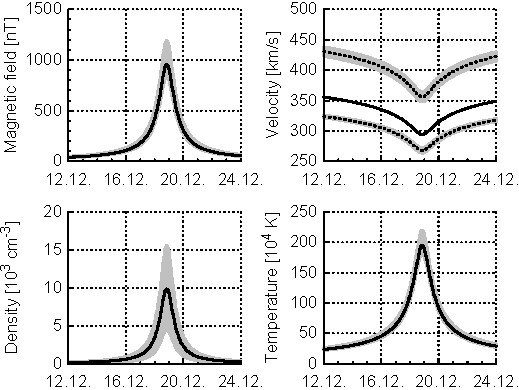
\includegraphics{figures/SPP_perihelia_prediction_nearest_e_plot.pdf}}
	\caption{Estimated solar wind parameter medians (black) and their error bands (grey) during during 12 days in 2024 with PSP's nearest perihelion at \SI{0.0459}{\au}. For the velocity the combined median is calculated and also the SSN independent slow and fast parts are plotted (dotted).}
	\label{fig:SPP_perihelia_prediction_nearest_e_plot}
\end{figure}

\subsection{Model validity and error sources}
\label{sec:model_validity_and_errors}

validity and estimation of error size outside of valid model range...\\
derive heliocentric distance depending error...\\

list simplifications/approximations...\\

error estimation for general model and extreme value tendencies\\

error sources:\\
- extrapolation\\
- lognormal model\\
- SSN variance\\

all estimates outside these boundaries are extrapolations with large uncertainties.\\

discuss high value zoom figures\\

The solar wind parameters vary with solar distance as well as with latitudinal separation from the heliospheric current sheet (HCS).\\
The OMNI data is time-shifted to the nose of the Earth's bow shock. This leads to yearly solar distance variations of \SI{>2}{\percent} (cite?) as the Earth orbits the Sun. Furthermore, its orbit within the ecliptic leads to a yearly variation of \SI{+-7.2}{\degree} in heliospheric latitude.\\
The HCS's position in latitude is highly variable around the solar equator \citep[p.~127~ff.?]{Schwenn1990}.\\

Error estimation over the year (seasonal/monthly) -> we expect variations to be less than 5~\%\\


%OMNI data is not corrected for solar distace. only available for 1-/5-min data\\

%[limited parameter ranges... (minV: 171~km/s; Schwenn1983)]\\


\section{Results and discussion}

list of results:\\
- empirical solar wind model for inner heliosphere within ecliptic\\
- low velocity at 0.0459~au\\
- slow/fast ratio SSN dependency\\
- application validity of lognormal distributions\\
--> B inversion of frequency distribution\\
---> magnetic field distribution's with distance increasing high value tail -> source are compression regions (why with density no increase?); look into Parker1958's B-field formula...\\
varying shape with distance is indicator for internal physical processes (mixing/turbulence...)\\

%solar wind -> structures\\
\citet{Balogh1999} p.~162~ff (origin and formation of CIRs in inner heliosphere with Helios data; latitude V dependence)\\
Balogh2009 (HMF review + inner heliosheath)\\
Aschwanden2004, p.~29\\

individual velocity part discussion -> there is no specific velocity threshold between slow and fast solar wind types, the velocity ranges of both types overlap.\\
Not only the slowest wind but also the fastest wind is expected to converge to the average speed (Sanchez-Diaz2016 p.~2835, using MHD-model -> very slow solar wind is continuation of slow wind) (because of interaction).\\

The ratio of both varies with solar activity, e.g. 3~years after maximum, polar coronal holes are observed to often have equatorial extensions (cite?). see and use \citet{Bougeret1984} p.~498...\\

larger influx from higher latitudes (see figure b))\\

In most studies the density distance dependence is assumed to scale with $r^{-2}$ (cites), assuming a constant velocity.\\


\section{Conclusions}

Further investigations should be done into structure extrapolations; outward extension of model to Mars seems feasable...\\

Further questions:\\
nearer to the Sun (at and below the source surface) the solar wind expansion in the ecliptic should be less spherical but more circular due to the influx from higher latitudes. => density exponent > -2\\
see Li2011 Fig.~1\\
% n	v
% -2.05	0.05
% -2	0
% -1.8	-0.2
% -1.5	-0.5


